\documentclass[a4paper,10pt]{article}

\usepackage{color}
\usepackage{graphicx}
\usepackage[utf8]{inputenc}
\usepackage[english]{babel}
\usepackage{multicol}
\usepackage[margin=1.5cm,headsep=2cm]{geometry}

\setlength{\columnsep}{1cm}


\begin{document}

\title {Comparision of Dijkstra & Bellman-ford Algorithm}
\author{Mir Mursalin Hossain}
\author{Resbi Anik}
\date{\today}

\begin{center}
\LARGE\textbf{Comparision of Dijkstra \& Bellman-ford Algorithm}
\vspace{.3cm}
\\
\begin{multicols}{2}
\large\textit{Mir Mursalin Hossain\\Roll 133047}
\\
\large\textit{Md. Resbi Anik\\Roll 133050}
\\
\end{multicols}
\small\textrm{Dept. of Computer Science \& Engineering}
\\
\vspace{.1cm}
\small\textrm{Rajshahi University of Engineering \& Technology}
\\
\vspace{1.5cm}
\end{center}

\begin{multicols}{2}

\section{Abstract}
Both Dijkstra and Bellman-ford algorithm are used to find the shortest path between two or more nodes. They have different characteristics. Both algorithms have advantages and limitations upon each other. They are generally used in different sectors like as networking and communication, transportation, system analysis, business sector etc. Here we will discuss about performances of both algorithms like as time complexity, space complexity and negative cycle checking. To compare the algorithms we will use C++ programming language. The analysis of comparison is given briefly.

\section{Introduction}
In general sense we can divide graph into two parts. One of them is weighted graph and another is un-weighted graph.
Shortest path problem means the problem of finding the shortest in graph from one vertex to another. "Shortest" may be least number of edges, least total weight etc. There are different kinds of shortest path algorithms which are given below:
\begin{enumerate}
  \item Single source shortest path Algorithm
  \item Single destination shortest path Algorithm
  \item All pair shortest path Algorithm
\end{enumerate}
In single source shortest path algorithm we will consider both directed and undirected graphs. In graph, all edges must have nonnegative weights and graph must be connected. In this paper , we are comparing time, space, cycle checking and other criteria of single source Dijkstra and Bellman-ford algorithm. For comparing complexity we are taking Big O notation as standard. Here cycle checking means capability of negative cycle detecting between both algorithms.


\section{General discussion on Dijkstra and Bellman-ford algorithm}
Primary deliberation of both algorithms are given beneath :-\
\subsection{Dijkstra algorithm}
Dijkstra algorithm is the method of choice for finding shortest paths in an edge-weighted or vertex-weighted graph. Given a particular start vertex s, it finds the shortest path from s to every other vertex in the graph, including your desired destination t. This means that the algorithm checks for the following condition:
\\\\d[u] + edge weight $d[u][v] < d[v]$
\\\\According to Dijkstra algorithm we can reach from node u to v if this condition is satisfied and the updated value of d[v] is equal to the summation of d[u] and edge weight of  node u and v.
\\\\\\
\textbf{\large Psudocode: Shortest Path - Dijkstra(G, s, t)}
\\\\
\\$known = {s}$
\\for $i = 1$ to n, $dist[i] = infinity$
\\for each edge (s, v), $dist[v] = w(s, v)$
\\$last = s$
\\while $(last = t)$
\\select vnext, the unknown vertex minimizing dist[v]
\\for each edge (vnext, x), $dist[x] = min[dist[x], dist[vnext] + w(vnext, x)]$
\\$last = vnext$
\\known = known U {vnext}
\\\\
\\Dijkstra is a greedy algorithm. It simply assumes that the path through v is the shortest because $d[v] < d[u]$. So each time after computing the path for a particular vertex, it is just added in the already obtained solution to the previous vertices in order to get the net distance from the origin vertex.\\\\

\textbf{\large Algorithm details about Dijkstra algorithm:}\\\\\\
Detailed steps used in Dijkstra’s algorithm to find the shortest path from a single source vertex to all other vertices in the given graph.
Algorithm\\\\
\textbf{1)} Create a set sptSet (s=shortest p=path t=tree set) that keeps track of vertices included in shortest path tree, i.e., whose minimum distance from source is calculated and finalized. Initially, this set is empty.\\
\textbf{2)} Assign a distance value to all vertices in the input graph. Initialize all distance values as INFINITE. Assign distance value as 0 for the source vertex so that it is picked first(initialization).\\\\
\textbf{3)} While sptSet doesn’t include all vertices\\\\
….\textbf{a)} Pick a vertex u which is not there in sptSet and has minimum distance value.\\\\
….\textbf{b)} Include u to sptSet.\\\\
….\textbf{c)} Update distance value of all adjacent vertices of u. To update the distance values, iterate through all adjacent vertices. For every adjacent vertex v, if sum of distance value of u (from source) and weight of edge u-v, is less than the distance value of v, then update the distance value of v.\\\\

\textbf{\large Example:}\\\\\\
\begin{figure}[h]
 \centering
  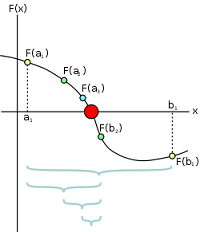
\includegraphics[width=1.5in]{bisect.png}
    \caption{Graphical representation of the bisection method \cite{r5}.}
  \label{fig:bisect1}
  \end{figure}

\end{multicols}
\end{document} 